\documentclass[FinalReport.tex]{subfiles}
\begin{document}

\section*{\textsc{\Large Results}}

An initial way to view the performance of the traces with specific configurations is to look at the execution times for those Configurations.  Fig.~\ref{fig:executiontimes} shows each Trace and its execution time for each Configuration in relation to all the other traces.
\begin{figure}[H]
\centering
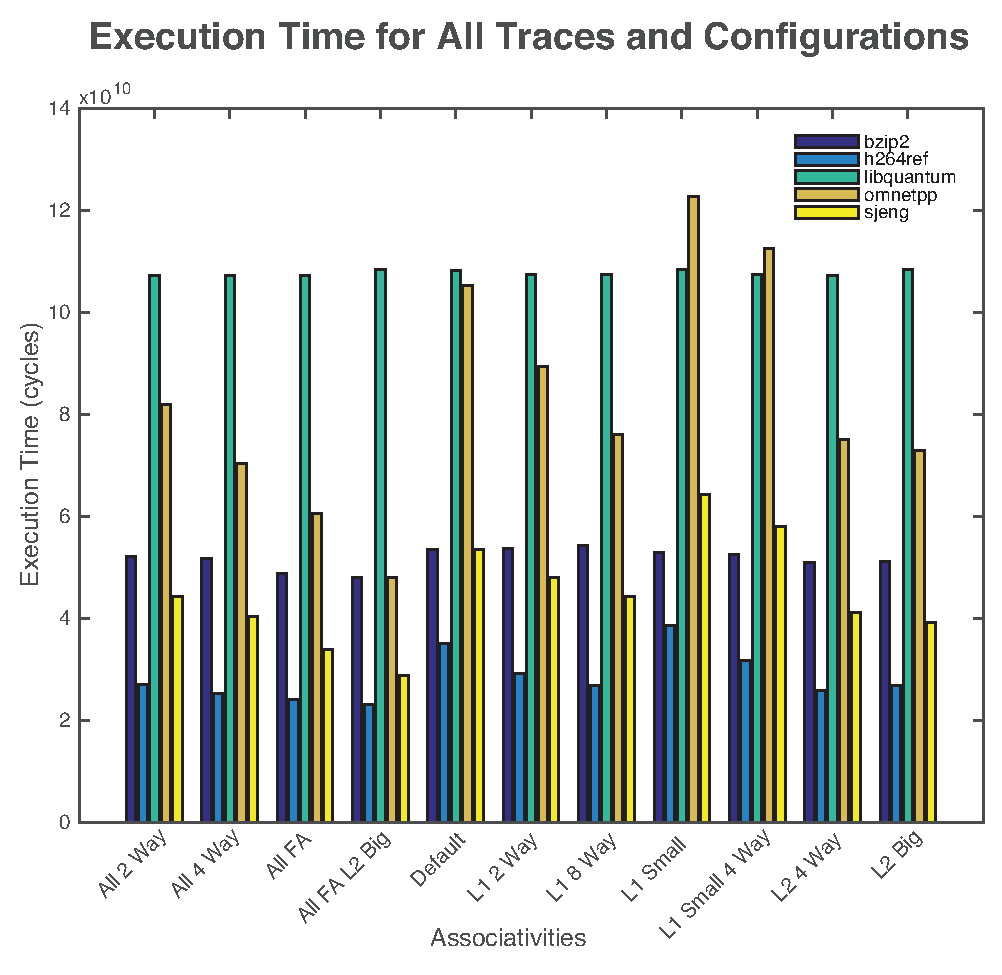
\includegraphics[scale = 0.65]{bargraph1.eps}
\caption{Execution times of all traces with correspondence to all configurations\label{fig:executiontimes}}
\end{figure}
The execution time for some traces varies very little with changes in cache configuration while other traces are largely effected by the cache configuration.  As seen in Fig.~\ref{fig:executiontimes}, {libquantum} has a very steady execution time which does not seem to depend on cache configuration.  A trace like {omnetpp} however, is very dependent on the cache configuration.  The execution times range from 40 billion cycles to 120 billion cycles. 

Another way to compare the performance of each trace is to look at the Cycles per Instruction (CPI).  This is plotted in Fig.~\ref{fig:CPI}.
\begin{figure}[H]
\centering
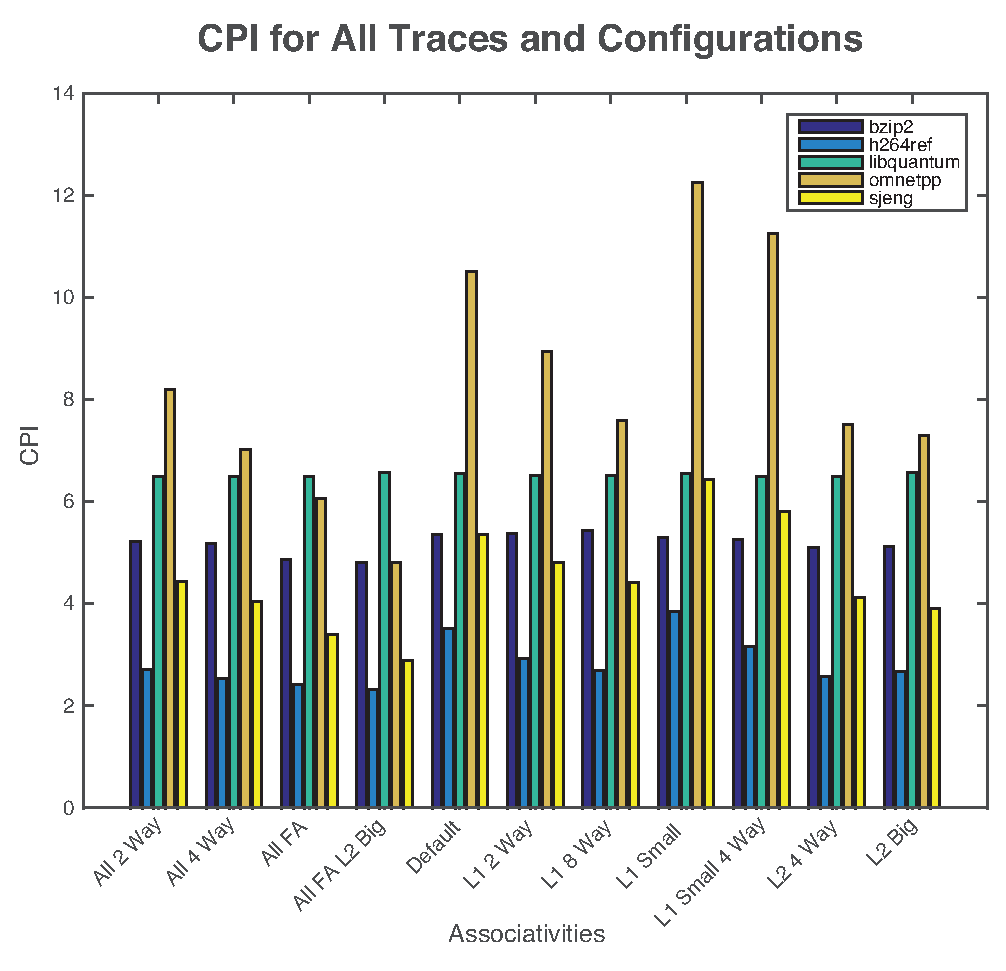
\includegraphics[scale = 0.65]{CPITimes.eps}
\caption{CPI of all traces with correspondence to all configurations\label{fig:CPI}}
\end{figure}

Similar to the execution times in Fig.~\ref{fig:executiontimes}, Fig.~\ref{fig:CPI} shows that the configuration of the cache can dramatically effect the CPI. 

Figures.~\ref{fig:executiontimes}~\&~\ref{fig:CPI} show that Fully Associative configurations give the fastest results, but at what cost
\begin{figure}[H]
\centering
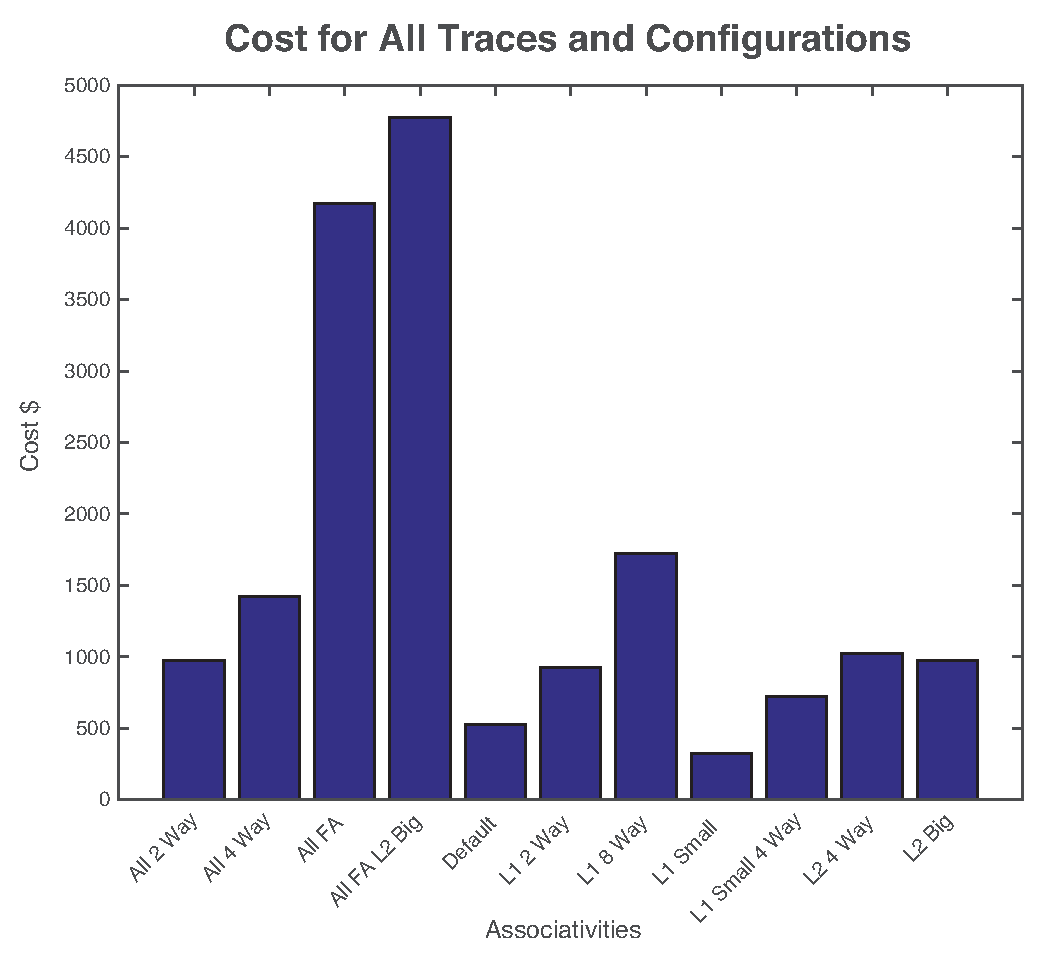
\includegraphics[scale = 0.75]{costVsConfig.eps}
\caption{Cost of all the different configurations\label{fig:costVsConfig}}
\end{figure}
Fig.~\ref{fig:costVsConfig} shows the total cost of having each configuration.  The fully associative configurations are much more expensive than the other configurations.  Viewing both Fig.~\ref{fig:CPI}~\&~\ref{fig:costVsConfig} show that cost transfers quite proportionally to performance.  

%The next step is to find the performance of the configurations with respect to the cheapest/slowest configuration.  It was found that L1 small was the cheapest and slowest (on average) configuration.  Fig.~\ref{fig:nextBest} shows the relative performance per dollar with respect to the L1 Small configuration.



%Fig.~\ref{fig:nextBest} uses Instructions per Cycle to calculate relative performance with respect to L1 Small.  

%\begin{figure}[H]
%\centering
%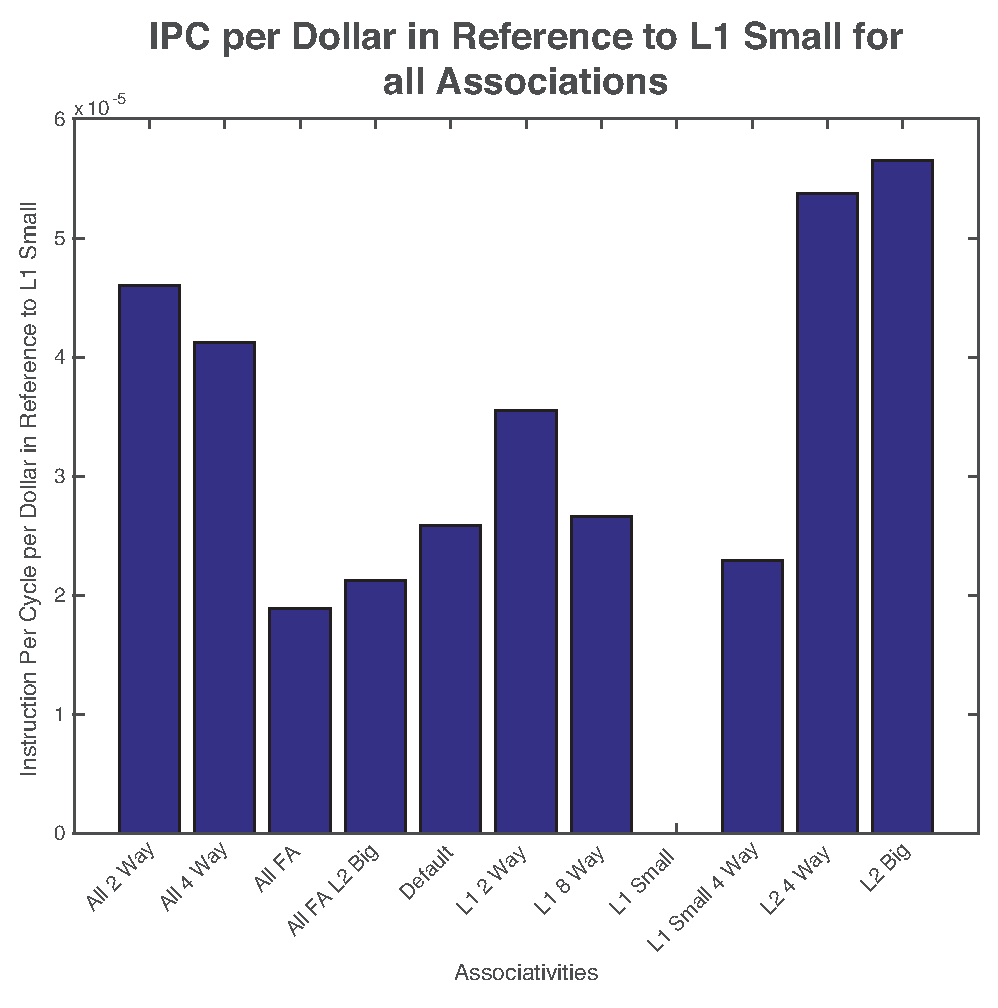
\includegraphics[scale = 0.75]{nextBest.eps}
%\caption{\label{fig:nextBest}}
%\end{figure}




\end{document}
